\section{Overview of CrowdNotifier}

We present CrowdNotifier. CrowdNotifier aims to help health authorities to implement presence tracing while being easy to use for users and being easy to deploy for venue owners and event organizers. Moreover, the system aims to be respectful of the following design principles, already implemented in decentralized contact tracing:

\begin{itemize}
\item \textit{Privacy by design}: no private/sensitive data should be stored in any central database. Moreover, private data should not be derivable from data (e.g., logs) that are stored for operational purposes.
\item \textit{Purpose limitation by design}: abusing the system for population control, location tracing, or other objectives other than sending notifications should be difficult if not impossible.
\item \textit{Voluntary basis}: Use of the digital system is not mandatory. A non-digital fallback must always be available.
\end{itemize}

We design the system under the following assumptions:

\begin{enumerate}
\item The health authorities has the means to identify which locations have been visited by a SARS-CoV-2-positive person, and at what times those visits happened.
\item The digital system can rely on the use of a mobile app on the user’s device. This app can be either separate or integrated with existing proximity tracing solutions. In either case, the system must be designed such that the privacy properties of both proximity and presence tracing  are guaranteed. The design proposed later on in this document fulfills this property.
\item Presence tracing should be possible even if the SARS-CoV-2-positive person did not themselves use the app.
\item Users can be trusted to follow notifications from the app, just like they would when they are notified of a close contact by a digital contact tracing app.
\end{enumerate}

The first assumption implies that CrowdNotifier does not need to provide means to identify which locations had a prolonged visit of a SARS-CoV-2-positive person. Just the means to notify other visitors that this even happened and they are at risk and need to take precautions.

The second assumption delimits the technological capabilities on which the design can rely: the kind of sensors that can be used, and the connectivity and the computational capabilities that can be expected.
The use of an app guarantees that the system can notify all visitors, even in the case in which the SARS-CoV-2-positive person did not themselves use the app. 

The third assumption supports the voluntary nature of the system. It is in line with the current approach used in many places, which assumes that visitors can put their actual phone numbers and name in an attendance log that can be provided to the authorities. There is empirical evidence that many fake numbers are used. In fact, one can reasonably expect better compliance from a privacy-preserving digital solution (where citizens should take action when actually exposed) vs. the classic solutions (where citizens should take action -- i.e, write down their real phone number -- when attending the venue).

The fourth assumption implies that there is no need to design an enforcement mechanism to ensure that notified users that receive a notification comply with the instructions they receive.

\subsection{A walkthrough of the system}
The following example illustrates the operation of the CrowdNotifier system. For illustration, we use a venue as location (e.g., an association’s meeting place, a mosque, a church, a meeting room, a bar, a restaurant, a night club), but we recall that a location could also represent an event that spans different locations (e.g., a demonstration). 

In \name users store encrypted records for each visit on their phone. These
records can only be decrypted using the decryption key for the corresponding
time slot. Without this key, these records reveal nothing, guaranteeing users'
privacy against strong attackers. To initiate tracing, the health authority -- together with the location owner -- computes and publishes the proper time-slot specific decryption keys. Apps regularly download these keys and use them to try to unlock the encrypted records. If encryption succeeds, the user may need to be notified.

To build this time-slot specific encryption system, \name uses an identity-based encryption (IBE) scheme. Each location owner acts as the trusted authority. In this setting, users store records of visits by encrypting against a time-based identity for the location they visit. The location owner with the health authority compute the corresponding identity-based decryption keys to enable tracing.

\paragraph{Setting up}
Suppose Charlie manages a location for which she decides to use \name presence notification to help her visitors break transmission chains after an outbreak. To do so, Charlie first uses \name to generate and print two QR codes: an \emph{entry code} and a \emph{tracing code}. The entry code contains information describing the venue as well as an identity-based master public key. The tracing code contains the corresponding master private key.

Charlie posts the entry code in a place where visitors can scan it (e.g., at the entrance, or on the tables), and keeps the tracing code private. See Figure~\ref{fig:overview}, Setup.

\paragraph{Visiting the location}
When entering the location, visitors can use the app or not. If they do, they scan the QR code posted at the entry to the location. The app shows the name of the location and asks the user to confirm the check in.
See Figure~\ref{fig:overview}, Entering a venue. If they do not use the app, they write their contact information on an attendee list.\footnote{The collection of non-digital data should also be made according to the data minimization principle. It suffices to provide contact information. For the purpose of notifying visitors, these visitors do not need to be identified.}

Once the app learns the departure time (e.g., because the user explicitly checks out after a reminder from the app), the phone stores a private record containing the identity-based encryption (using the location's master public key) of the entry and departure times, using the entry hour as part of the identity.
Our choice of identity-based encryption scheme ensures that these ciphertexts do not reveal the location for which they were created to anyone with access to the user's phone as long as the location owner does not compute and reveal the specific decryption key.


\begin{figure}
  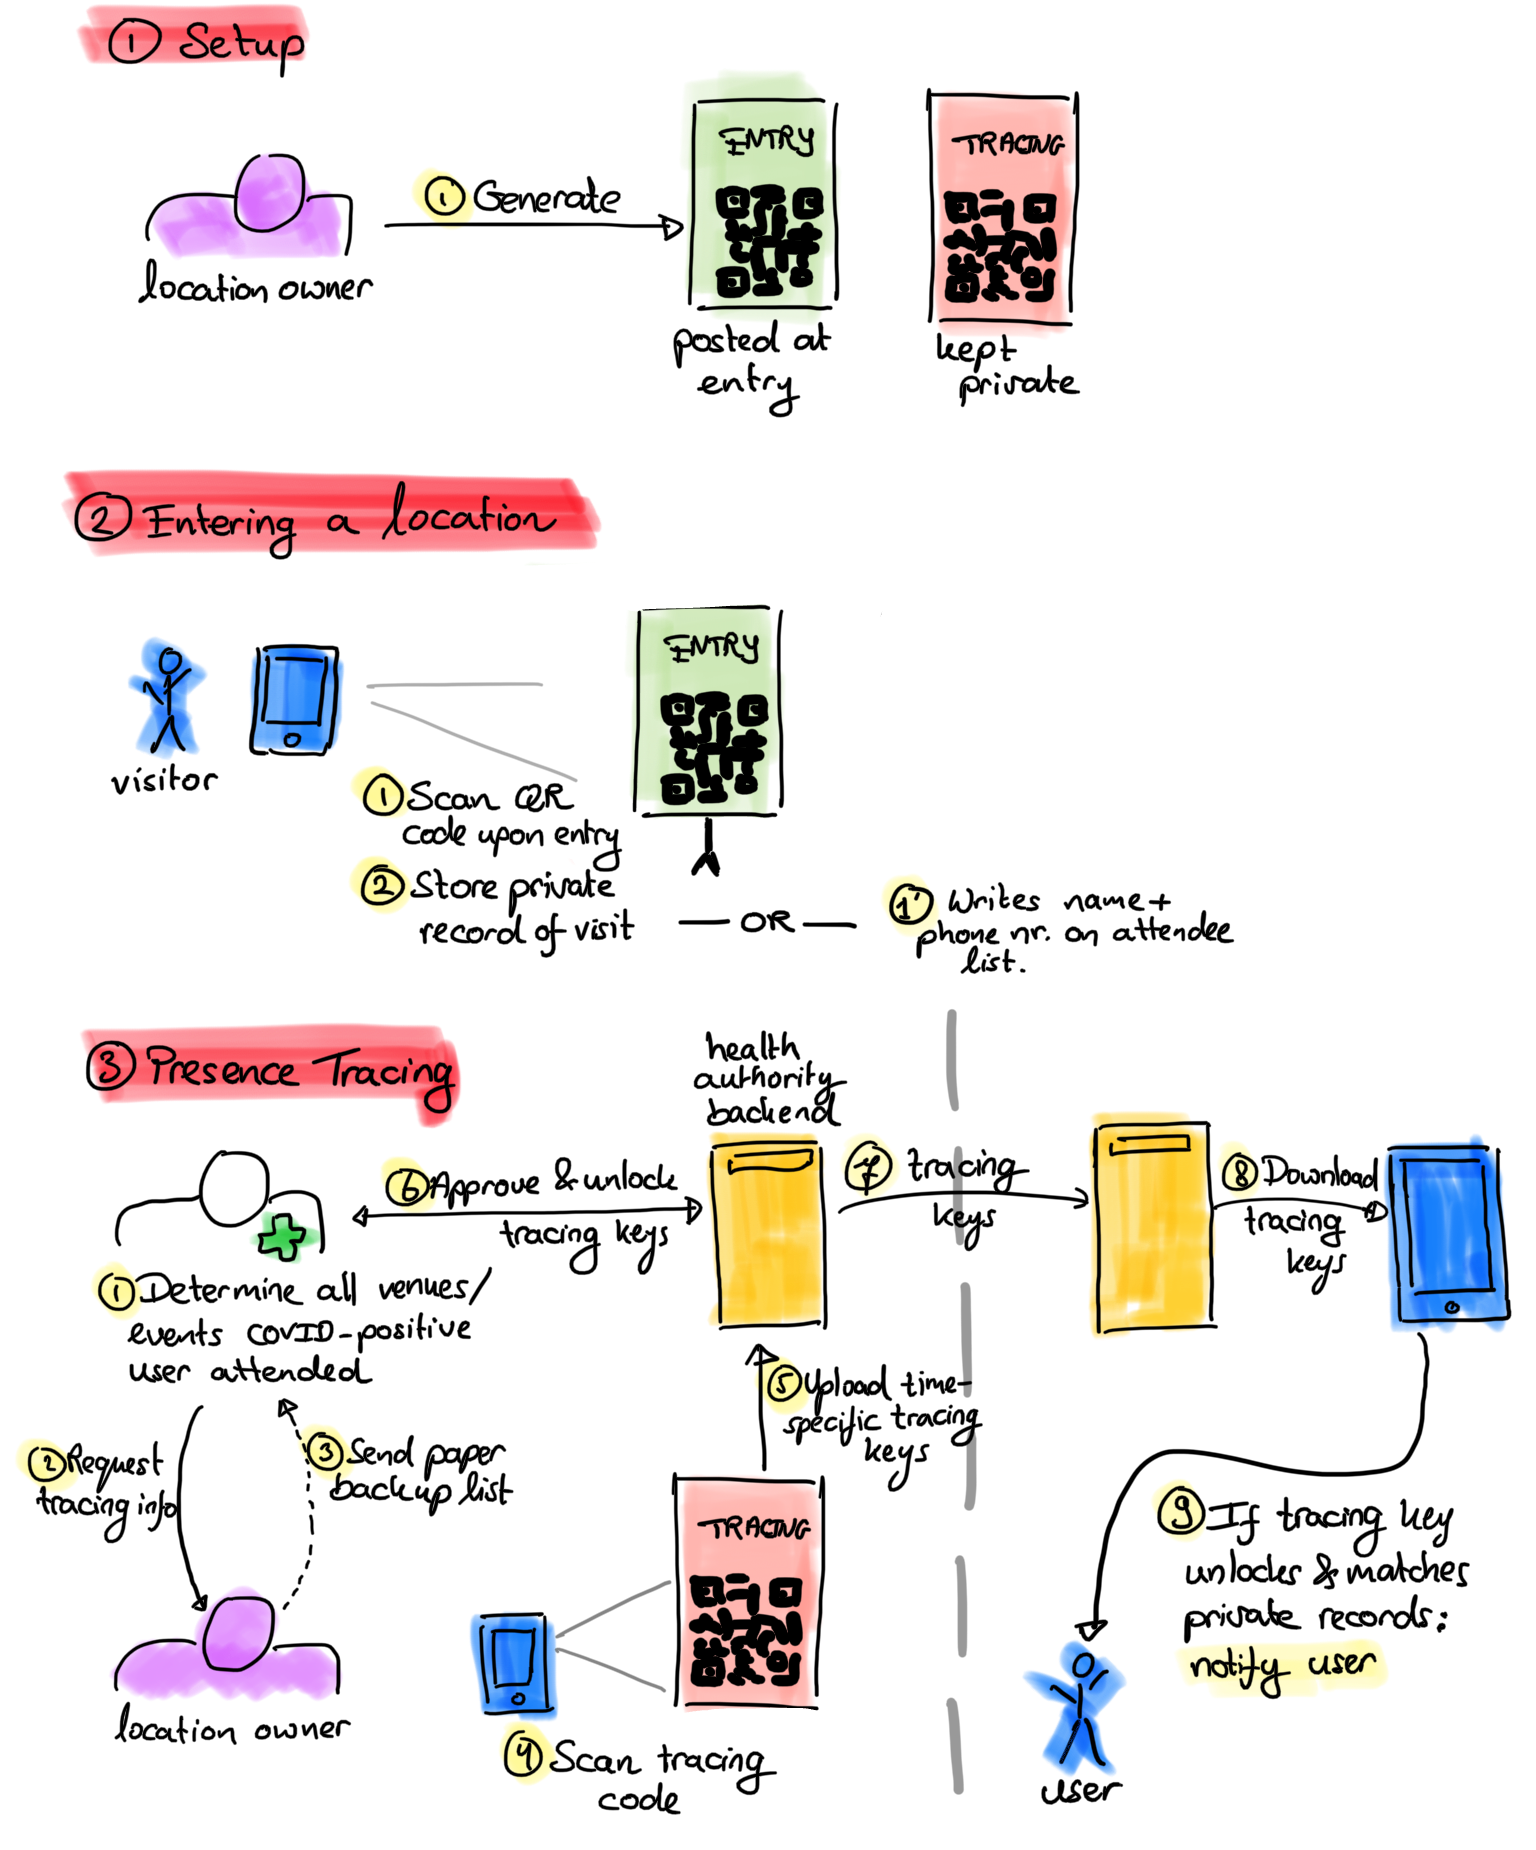
\includegraphics[width=\textwidth]{figures/overview2}
  \caption{\label{fig:overview}Overview of the core operations in our proposal for Presence Tracing}
\end{figure}

\paragraph{Presence tracing}
First, health officials need to determine which locations the SARS-CoV-2-positive person attended (step 1, Figure~\ref{fig:overview}, Presence Tracing), e.g., using the traditional interviewing process in which different positive users report having been at a location. The health official then contacts the owner for each of these locations, requesting two things (step 2):

\begin{itemize}[topsep=0pt, partopsep=0pt]
\item The paper backup list (step 3)
\item That the location owner uploads tracing keys, i.e., identity-based decryption keys, for the affected time interval (steps 4 and 5).
\end{itemize}

The health official checks and approves the uploaded tracing keys (step 6). This ensures that the data corresponds to the requested location. Then, the health authority’s backend makes available the tracing keys (steps 7 and 8) to all users of the system. 

Phones download the provided tracing keys to try and unlock (i.e., decrypt) private records stored on the phone. If unlocking succeeds, it means that the user was at a location with a SARS-CoV-2-positive person. In this case, the phone recovers the user's entry and departure times for the venue. The phone then determines if there is an epidemiologically relevant overlap between the user’s time at the location and that of the SARS-CoV-2-positive person. If there is, the phone notifies the user (step 9).
